\documentclass[11pt,a4paper]{article}
\usepackage[margin=2cm]{geometry}                % See geometry.pdf to learn the layout options. There are lots.
\geometry{a4paper}                   % ... or a4paper or a5paper or ... 
%\geometry{landscape}                % Activate for for rotated page geometry
%\usepackage[parfill]{parskip}    % Activate to begin paragraphs with an empty line rather than an indent
\usepackage{graphicx}
\usepackage{amssymb}
\usepackage{epstopdf}
\usepackage{tabularx}
\usepackage{booktabs}
\usepackage{textcomp}
\usepackage{libertine}
\usepackage{float}
\usepackage{tikz}
\usepackage{nopageno}

\begin{document}

{\Huge Oxford Oscillations Meeting}

3-5 September 2017, St Catherine's College, Oxford, UK.

Supported by the James S. McDonnell Foundation

\vspace{1cm}
\parbox{.85\textwidth}{\raggedright All talks and coffee breaks will take place at St Catherine's College in the Mary Sunley Building. Lunch is served in the College Hall. Departure to dinner on Saturday and Monday will be from the St Catherine's College Porter's Lodge. Wifi access is available through ``eduroam`` or ``TheCloud`` (requires free registration).}

\vspace{1cm}
 %%%%%%%%%%%%%%%%%%%%%%%%%%%%%%%%%%%%%%%%%
\begin{figure}[h]
\centering
\begin{tabularx}{.95\textwidth}{l p{.8\linewidth}}
\multicolumn{2}{l}{\Large Saturday 2nd September }\\
\toprule
& {\bf Arrival during afternoon/evening}\\
19.00 & Departure from St Catherine's for dinner\\
19.30 & Dinner at {\it My Sichuan}\\
%\bottomrule
\end{tabularx}
\end{figure}
 %%%%%%%%%%%%%%%%%%%%%%%%%%%%%%%%%%%%%%%%%
\begin{figure}[h]
\centering
\begin{tabularx}{.95\textwidth}{l p{.8\linewidth}}
\multicolumn{2}{l}{\Large Sunday 3rd September }\\
\toprule
9:00 & Opening Remarks \\
\\
9:10 & {\bf Cognition}\vspace{.25cm} \\
     & \parbox{.85\textwidth}{\raggedright\small9:10 \phantom{0}{\bf Beth Buffalo} - Active Sensing and Oscillatory Activity in the Primate Hippocampus}\vspace{.15cm}\\
& \parbox{.8\textwidth}{\raggedright\small 10:00 {\bf Freek van Ede} -What human alpha and beta oscillations tell us about attentional dynamics in visual working memory}\vspace{.15cm}\\
& \parbox{.85\textwidth}{\raggedright\small 10:50 Coffee }\vspace{.15cm}\\
& \parbox{.85\textwidth}{\raggedright\small 11:20 {\bf Miles Whittington} - Theta/Delta Cross-Frequency Coupling Underlies Semantic Decision Making}\vspace{.15cm}\\
& \parbox{.85\textwidth}{\raggedright\small 12:10 {\bf Discussion} - Chair: Sabine Kastner}\vspace{.15cm}\\
\\
13:00 & Lunch (in hall) \\
\\
14:30 & {\bf Methods \& Mechanisms}\vspace{.25cm} \\
& \parbox{.85\textwidth}{\raggedright\small 14:30  {\bf Nancy Kopell} - Coordination and Modulation of Brain Rhythms}\\
& \parbox{.85\textwidth}{\raggedright\small 15:20 Coffee }\vspace{.15cm}\\
\\
& {\raggedright\small 15:50 Keynote by {\bf Norden Huang} National Central University}\\
& \parbox{.85\textwidth}{\small  \hspace{2.5cm} Holo-spectral Analysis: From Turbulence to Brain Waves}\\
\\
& \parbox{.85\textwidth}{\raggedright\small 17:00 {\bf Discussion} - Chair: Ole Jensen}\\
\\
17:00 & Close\\
19:30 & Drinks Reception (Mary Sunley Seminar Room)\\
20:00 & Dinner in St. Catherine's Senior Common Room\\
%\bottomrule
\end{tabularx}
\end{figure}
 %%%%%%%%%%%%%%%%%%%%%%%%%%%%%%%%%%%%%%%%%
\begin{figure}[h]
\centering
\begin{tabularx}{.95\textwidth}{l p{.8\linewidth}}
\multicolumn{2}{l}{\Large Moday 4th September }\\
\toprule
9:10 & {\bf Gamma Oscillations}\vspace{.25cm} \\
& \parbox{.85\textwidth}{\raggedright\small 9:10 \phantom{0}{\bf Jess Cardin} - Interneuron Control of Cortical Rhythms}\vspace{.15cm}\\
& \parbox{.8\textwidth}{\raggedright\small 10:00 {\bf  John Lisman} - Evidence for a Theta-Gamma Phase Code in Working Memory: Specific Functions of Theta and Gamma Oscillations}\vspace{.15cm}\\
& \parbox{.85\textwidth}{\raggedright\small 10:50 Coffee }\vspace{.15cm}\\
& \parbox{.85\textwidth}{\raggedright\small 11:20 {\bf Vitor Lopez de Santos} - Single-cycle profiling of hippocampal theta oscillations suggest transient network states }\vspace{.15cm}\\
& \parbox{.85\textwidth}{\raggedright\small 11:40 {\bf Marcin Leszczynski} - Dissociation of broadband high-frequency activity and neuronal firing}\vspace{.15cm}\\
& \parbox{.85\textwidth}{\raggedright\small 12:10 {\bf Discussion} - Chair: David Dupret}\vspace{.15cm}\\
\\
13:00 & Lunch (in hall) \\
\\
14:30 & {\bf Excursion in Oxford}\\
& Either punting from New College or visit to the Pitt Rivers\\
\\
19:00 & Departure from St Catherine's for Cherwell Boathouse\\
19:30 & Dinner at Cherwell Boathouse\\
%\bottomrule
\end{tabularx}
\end{figure}
 %%%%%%%%%%%%%%%%%%%%%%%%%%%%%%%%%%%%%%%%%
\begin{figure}[H]
\centering
\begin{tabularx}{.95\textwidth}{l p{.8\linewidth}}
\multicolumn{2}{l}{\Large Tuesday 5th September }\\
\toprule
9:30 & {\bf Entrainment}\vspace{.25cm} \\
& \parbox{.85\textwidth}{\raggedright\small 9:30 \phantom{0}{\bf Ayelet Landau} - Attentional Sampling: A Human Exploration Mechanism}\vspace{.15cm}\\
& \parbox{.85\textwidth}{\raggedright\small 10:20 {\bf Saskia Haegens} - Rhythmic facilitation of temporal attention.}\vspace{.15cm}\\
& \parbox{.85\textwidth}{\raggedright\small 11:10 Coffee }\vspace{.15cm}\\
& \parbox{.85\textwidth}{\raggedright\small 11:40 {\bf Flavio Fr{\"o}hlich} - Targeting Brain Oscillations}\vspace{.15cm}\\
& \parbox{.85\textwidth}{\raggedright\small 12:30 {\bf Discussion} - Chair: Charlie Schroeder}\vspace{.15cm}\\
\\
13:00 & Close \\
\\
& \hrulefill
\\
 & {\bf James S. McDonnell Postdoc Meeting}\\
 \\
13:00 & Lunch (in hall) \\
\\
14:00 & {\bf Meeting}\\
& \parbox{.85\textwidth}{\raggedright\small 14:00 {\bf Overview \& Catch-up Talks} }\\
& \parbox{.85\textwidth}{\raggedright\small 15:00 {\bf Theory \& Big Picture Discussion} }\\
& \parbox{.85\textwidth}{\raggedright\small 16:00 Coffee }\\
& \parbox{.85\textwidth}{\raggedright\small 16:30 {\bf Experimental Discussion}}\\
& \parbox{.85\textwidth}{\raggedright\small 17:00 {\bf Practical Discussion}}\\
\\
17:30 & Close\\
19:00 & JSMF Dinner\\
%\bottomrule
\end{tabularx}
\end{figure}




\pagebreak

\newgeometry{left=5cm,bottom=0.1cm}
{\Large Participants in no particular order} - (s) indicates a speaker
\begin{figure}[H]
\centering
\begin{tabularx}{.95\textwidth}{l p{.8\linewidth}}

Kia Nobre & Oxford\\
Charlie Schroeder & Columbia / NKI \\
Ole Jensen & Birmingham\\
Sabine Kastner & Princeton\\
Bob Knight & Berkeley\\

Beth Buffalo & U Washington (S)\\
Jessica Cardin & Yale (S)\\
Flavio Fr{\"o}hlich & U North Carolina (S)\\
Saskia Haegens & Columbia / NYU (S)\\
Norden Huang & National Central University, Taoyuan (S)\\
Nancy Kopell & Boston University (S)\\
Ayelet Landau & Hebrew University Jerusalem (S)\\
John Lisman & Brandeis (S)\\
Freek van Ede & Oxford (S)\\
Miles Whittington & York (S)\\
Marcin Leszczynski & Columbia (S)\\

arlies Vissers & Birmingham\\
Tjerk Gutteling & Birmingham\\
Idan Tal & Columbia\\
Marcin Leszczynski & Columbia\\
Anne Martin & Princeton\\
Tim Buschman & Princeton\\
Chi-Hung Juan & National Central University, Taoyuan\\

Lauren Atkinson & Oxford\\
Anna-Katharina Bauer & Oxford\\
Robert Becker & Oxford\\
Sage Boettcher & Oxford\\
Sven Braeutigam & Oxford\\
Peter Brown & Oxford\\
Sammi Chekroud & Oxford\\
David Dupret & Oxford\\
Simone Heideman & Oxford\\
Vitor Lopez de Santos & Oxford\\
Nick Myers & Oxford\\
Magdalena Nowak & Oxford \\
Andrew Quinn & Oxford\\
Eelke Spaak & Oxford\\
Mark Stokes & Oxford\\
Diego Vidaurre & Oxford\\
Catharina Zich & Oxford\\
Nahid Zokaei & Oxford\\
\end{tabularx}
\end{figure}
\restoregeometry
\pagebreak

\newgeometry{left=1cm,right=1cm,top=2cm,bottom=0.1cm}
\begin{figure}[htbp] %  figure placement: here, top, bottom, or page
   \centering
\begin{tikzpicture}
\node[inner sep=0pt] (russell) at (0,5)
    {\Large Maps of Oxford \& St Catherine's College};
\node[inner sep=0pt] (russell) at (0,0)
    {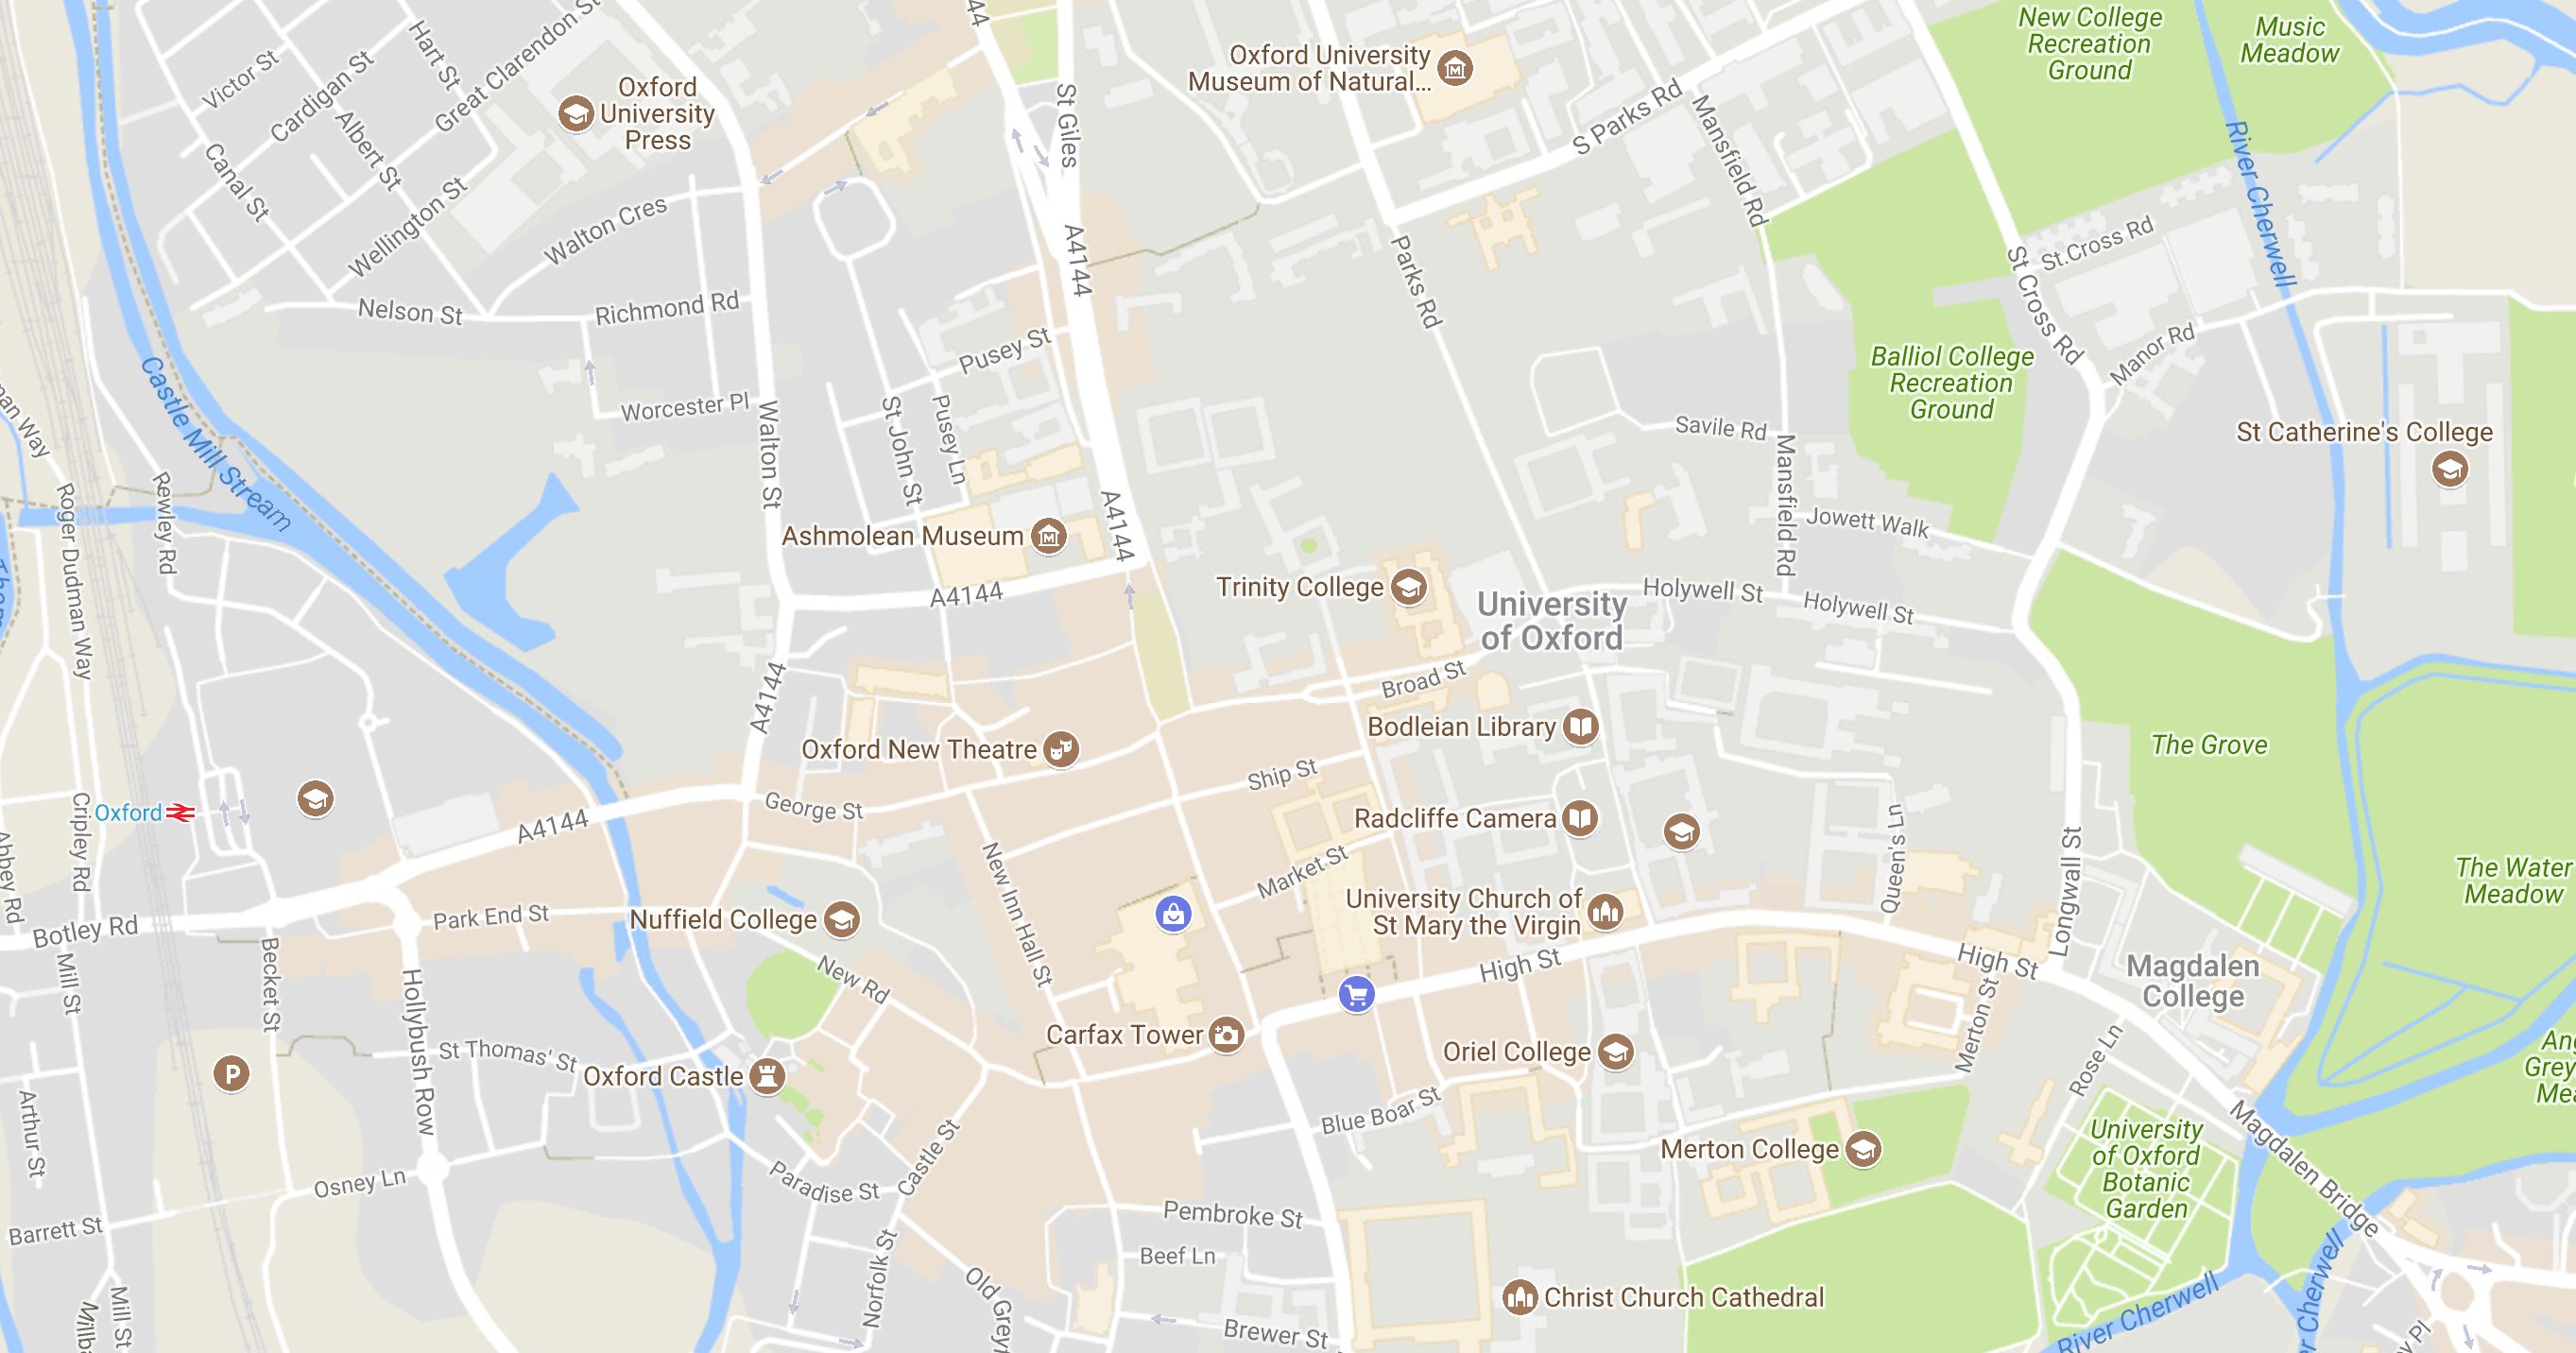
\includegraphics[width=.9\textwidth]{oxford_googlemaps.png}};

\node[inner sep=0pt] (russell) at (0,-11)
    {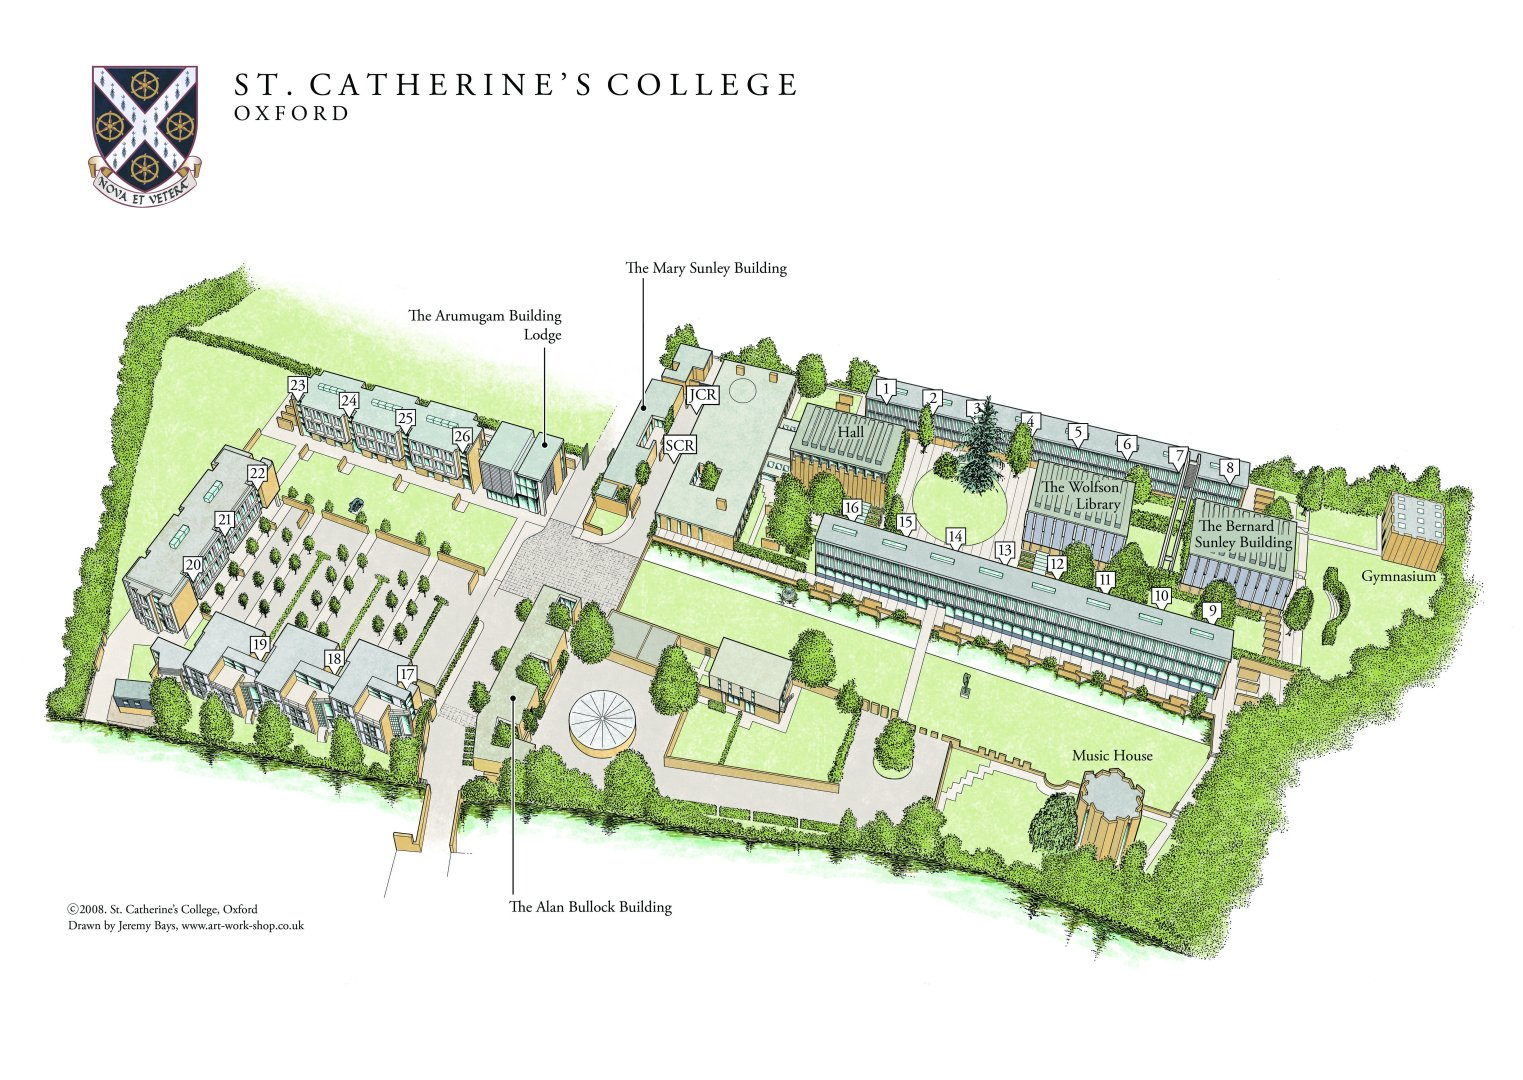
\includegraphics[width=1\textwidth]{campus.jpg}};
\end{tikzpicture}
\end{figure}
\restoregeometry

\end{document}
